% Response to Editor
% todo 改成Prof. / Dr. Cui
\editor

% todo complete

% ? 放原文吗

\begin{metacomment}
	Clearly differentiate the contributions from prior works.
\end{metacomment}
\begin{metaresponse}
\end{metaresponse}% todo 修改 appreciate
	We appreciate your handling of the review process.
	Compared with previous works, our current further considers the complex overlapping or containing range relationship between sensors.
	We have revised Section 1 to better highlight the challenge introduced by this relationship and to underscore their practical relevance in real-world scenarios.
	
	The revised description of this relationship and the associated challenge are given below, respectively.
	\begin{changes}
		This altitude-dependent coverage creates intricate spatial relationships between sensors, manifesting in various overlapping patterns: partial overlap, full containment, reverse containment, and disjointness.
		Moreover, these relationships become even more complex as communication range changes with altitude, creating challenges that have not been fully addressed in previous research.
		For example, in Fig.~1, as the altitude increases, sensor $S_1$ initially overlaps with $S_2$, but eventually becomes fully contained by $S_2$.
		Such overlapping range relationship better captures the complexity of real-world scenarios and provides practical value for UAV-assisted data collection.
		Capturing and fully exploiting these altitude-dependent ranges is crucial, since it enables the data from a single sensor to be collected across multiple sessions and fundamentally influences the order of data collection.
	\end{changes}
	\begin{changes}
		Due to the complex overlapping patterns of sensor data transmission ranges, the UAV is often simultaneously located within the ranges of multiple sensors. Consequently, determining the optimal data collection sequence becomes highly challenging.
	\end{changes}
\begin{metacomment}
	Address limitations for practical application of the algorithm.
\end{metacomment}
\begin{metaresponse}% todo 修改 appreciate
	
\end{metaresponse}

\begin{metacomment}
	Validate the claim of ``near-optimal performance.''
\end{metacomment}
\begin{metaresponse}% todo 修改 appreciate
	We appreciate the reviewers' insightful comment.
	We recognize that the term ``near-optimal'' was not precise. Our intention was to indicate that SSF-ACO-Online performs closely to the offline algorithm SSF-ACO. We have revised the abstract to clarify this point and removed the term ``near-optimal'' to avoid confusion.
	\begin{changes}
		Extensive simulations demonstrate that SSF-ACO significantly outperforms baseline approaches in energy efficiency, and SSF-ACO-Online achieves comparable performance with energy consumption 1.24\% higher than offline counterpart in average.
	\end{changes}
\end{metaresponse}

\begin{metacomment}
	Test SSF-ACO and SSF-ACO-Online under network dynamics (e.g., node mobility).
\end{metacomment}
\begin{metaresponse}% todo 修改 appreciate
	
\end{metaresponse}

\begin{metacomment}
	Explain the rationale behind heuristic factor selection.
\end{metacomment}
\begin{metaresponse}% todo 修改 appreciate
	We appreciate the reviewers' comment.
	In the algorithm, $\alpha$ and $\beta$ are the exponential parameters to control the influence of pheromone and heuristic values, respectively.
	We performed a grid-search over representative combinations of the pheromone exponential factor $\alpha\in\{1,2,3,4\}$ and heuristic exponential factor $\beta\in\{0,1,2,3,4\}$ to access parameter sensitivity as shown in Figure~\ref{meta:fig:cali}.
	The algorithm's performance under $\beta=0$ is significantly worse than performance for other parameter combinations. $\beta=0$ eliminates the use of heuristic information, resulting in purely random exploration during the initial iterations and thus poor performance.
	The results also indicate that the configuration $\alpha=1,\beta=2$ consistently achieves the minimum energy consumption. Accordingly, we adopted $\alpha=1,\beta=2$ in all simulation experiments.
	\begin{figure}[h]
		\centerline{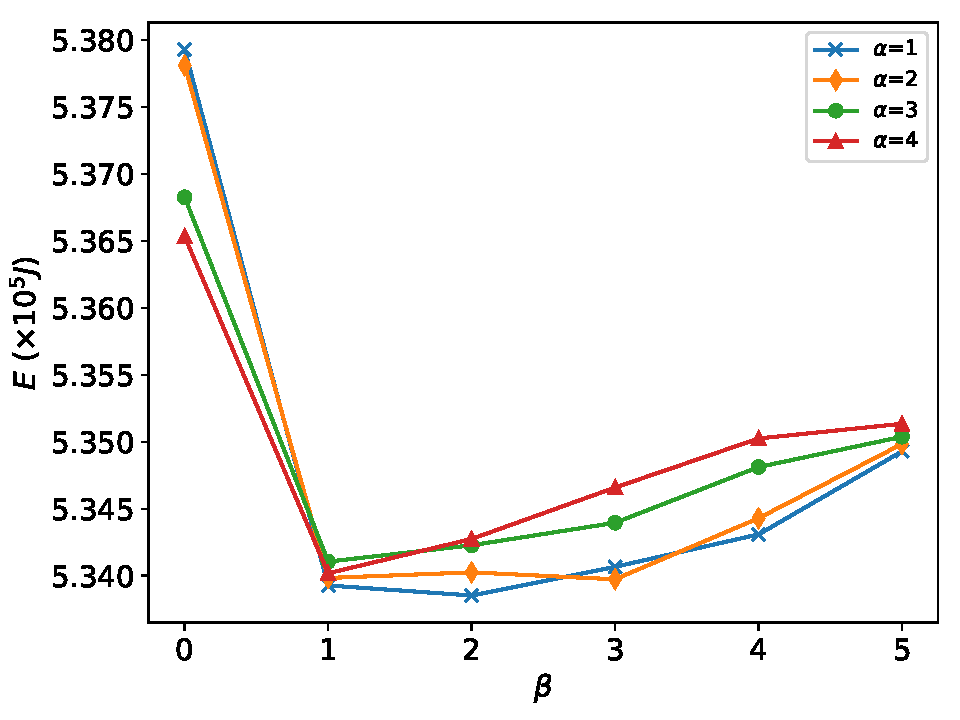
\includegraphics[width=.5\textwidth]{fig/cali.pdf}}
		\caption{Performance of SSF-ACO across different $(\alpha,\beta)$ combinations.}
		\label{meta:fig:cali}
	\end{figure}
\end{metaresponse}

\begin{metacomment}
	Include more comprehensive experimental validation.
\end{metacomment}
\begin{metaresponse}% todo 修改 appreciate
	
\end{metaresponse}

\begin{metacomment}
	Extend the discussion of related literature for completeness.
\end{metacomment}
\begin{metaresponse}% todo 修改 appreciate
	We appreciate the reviewers' suggestion.
	We have extended the discussion of related literature in the revised manuscript, especially in Section 2.3 regarding optimization algorithms for UAV-assisted systems.
	Popular algorithms are divided into three categories, including mathematical optimization techniques, heuristic algorithms, and learning-based methods. Their limitations are discussed.
	The revised Section 2.3 is as follows:
	\begin{changes}
		The optimization of UAV-assisted systems has attracted significant research attention, with various algorithms proposed to minimize energy consumption. 
		These approaches can be classified into three main categories.

		Mathematical optimization techniques were applied when the problem structure allowed theoretical analysis. 
		For instance, Shan \etal~\cite{SLXWL-INFOCOM20} derived optimal policies for linear data collection by constructing temporal-spatial constraints. 
		Other works~\cite{b-math1,b-math2} employed successive convex approximation for non-convex problems. 
		However, these methods often imposed strict assumptions on problem formulation and could be computationally intensive.

		Learning-based methods, particularly deep learning (DL) and RL, gained popularity in recent years, as they learned complex parameters or action policies during the training process.
		In UAV-assisted mobile edge computing systems, Lin \etal~\cite{b-DL} proposed a parametrized dueling deep Q-network to maximize the UAV's energy efficiency.
		The problem was formulated as a mixed-integer nonlinear programming (MINLP) problem, which facilitated the modeling of problems involving both continuous variables (\eg trajectory) and discrete variables (\eg data collection decision and task offloading decision).
		To maximize the total throughput and energy efficiency, Chen \etal~\cite{b-RL} formulated long-term UAV-aided data collection problem as a Markov Decision Process (MDP), and addressed it by a multi-agent DRL algorithm.
		However, the maximum number of ground nodes that could be served in \cite{b-DL} and \cite{b-RL} was only 6 and 8, respectively, as the extremely high computational complexity became unacceptable when the number of ground nodes increased.
		Hao \etal~\cite{hao-minlp} formulated a task offloading problem in a UAV-assisted mobile edge computing system as a MINLP, and then transformed it into a MDP.
		The problem was solved by a DRL algorithm.
		Zhong \etal~\cite{zhong-minlp} also applied a similar approach to address a task offloading and resource allocation problem.
		Despite their successful application to larger-scale problems, challenges still remain in the context of the JUSAS problem, particularly in modeling the environment and designing the reward function, including aligning the reward signal with the objective and dealing with sparse rewards.

		Heuristic algorithms were widely applied due to their greater flexibility and practical applicability.
		Fu \etal~\cite{a-heuristic1} considered a mobile crowdsensing scenario where UAVs collected data from mobile devices, and proposed a lightweight heuristic navigation algorithm to optimize UAVs' trajectory.
		The authors employed multiple virtual search agents to iteratively seek a satisfactory destination.
		Similarly, Lin \etal~\cite{a-heuristic3} developed a heuristic hexagon-based scheduling algorithm to improve eneryg efficiency for periodic data collection using UAVs,
		and also proposed an emergent node charging scheduling method to prevent node exhaustion.
		To reduce cost, Gong \etal~\cite{a-heuristic2} incorporate particle swarm optimization (PSO) algorithm to minimize the number of UAVs required to visit all sensors.
		Other meta heuristic algorithms included genetic-based algorithms~\cite{a-heuristic4} and simulated annealing (SA) algorithm~\cite{liao2024energy}.
		However, these methods are not readily applicable to the JUSAS problem.
	\end{changes}
\end{metaresponse}

% ? 需要吗
\printpartbibliography{SLXWL-INFOCOM20,b-math1,b-math2,b-DL,b-RL,hao-minlp,zhong-minlp,a-heuristic1,a-heuristic2,a-heuristic3,a-heuristic4,liao2024energy}
